\part{Geometry}
\chapter{Synthetic Geometry}
\section{Angles}
The reader should be familiar with terms such as segment, endpoint, midpoint, ray, origin, line, collinear.
\subsection{Phantom Points}

\section{Triangle}
\subsection{Triangle Centers}
\subsubsection{Definitions}
Let $ABC$ be a triangle. 

Triangle centers:
\begin{enumerate}
    \item Centroid $G$: Intersection of medians.
    \item Circumcenter $O$: Center of the circle which passes through vertices of the triangle.
    \item Incenter $I$: Intersection of the internal angle bisectors, which is also the center of the unique circle inside the triangle tangent to all three sides.
    \item Excenter $J$: Center of the circle which is tangent to sides of the triangle but lies outside the triangle.
    \item Orthocenter $H$: Intersection of altitudes.
\end{enumerate}

Associated inscribed triangles:
\begin{enumerate}
    \item Intouch triangle: The triangle whose vertices are the contact points of the incircle with the sides of $ABC$.
    \item \textbf{Medial triangle}: The triangle whose vertices are the midpoints of the sides of $ABC$.
    \item \textbf{Orthic triangle}: The triangle whose vertices are the feet of the altitudes.
\end{enumerate}

\subsubsection{Properties}
Centroid
medians cut triangle into 6 parts of equal area
G divides medians into segments of ratio 2:1

Circumcenter
R = a/2sinA = b/2sinB = c/2sinC

Incenter
r=area/s (s is semiperimeter)

Orthocenter
cyclic quadrilaterals
H,A,B,C are incenter/excenters of orthic triangle

Point where angle bisector of A meets perp bisector of BC lies on circumcircle of ABC. This point is also the center of circle passing through $B,C,I,J_A$

Properties of the orthocenter

\subsection{Right triangle}
\begin{thrm}{Pythagoras' Theorem}{}
For triangle $\triangle ABC$ where the right angle is at $\angle C$,
\begin{equation}
a^2+b^2=c^2
\end{equation}
\end{thrm}

Using similar triangles, we can deduce
\begin{equation}
\frac{1}{h^2}=\frac{1}{a^2}+\frac{1}{b^2}
\end{equation}
where $h$ is the perpendicular distance from $C$ to $a$.

\subsection{Congruency and Similarity}
Triangle similarity
\begin{enumerate}
    \item Two angles match.
    \item Two sides have lengths in the same ratio, and the angle between those two sides matches.
    \item Three sides have lengths in the same ratio.
    \item The triangles are right-angled and the ratio between one side and hypotenuse is the same.
\end{enumerate}

Triangle congruence
Same conditions but check that one corresponding side matches.

\subsection{Viviani's Theorem}
\begin{thrm}{Viviani's Theorem}{}
The sum of the distances from any interior point to the sides of an equilateral triangle equals the length of the triangle's altitude. 
\end{thrm}

\begin{proof}

\end{proof}

\begin{thrm}{}{}
The sum of the distances from any point P inside a parallelogram is independent of the location of P.

The converse also holds: If the sum of the distances from a point in the interior of a quadrilateral to the sides is independent of the location of the point, then the quadrilateral is a parallelogram.
\end{thrm}

\begin{thrm}{}{}
Generalisation: In a 2k-sided polygon with opposite sides parallel, the sum of distances from an arbitrary point inside the polygon to its sides is constant and is independent of the point's position.
\end{thrm}


Regular polygons:
Theorem 4. In every regular polygon, the sum of distances from an arbitrary point
inside the polygon to its sides is constant and is independent of the point's position.

Theorem 5. The sum of distances from a point to the side lines of an equiangular
polygon does not depend on the point and is that polygon's invariant.

% https://www.plmgss.moe.edu.sg/files/2020%20SMPF%20-%20Vivianis%20Theorem%20and%20Related%20Problems.pdf
\begin{thrm}{Carnot's Theorem}{}
For a triangle $ABC$, $P$ lies in the interior of the triangle. $D,E,F$ denote the foots of perpendicular from $P$ to sides $BC,CA,AB$ respectively. The following equation holds:
\begin{equation}AE^2 + BD^2 + CF^2 = AF^2 + BE^2 + CD^2\end{equation}
\end{thrm}

\begin{figure}[H]
    \centering
    \begin{tikzpicture}[dot/.style={circle,inner sep=1pt,fill,label={#1},name=#1},
  extended line/.style={shorten >=-#1,shorten <=-#1},
  extended line/.default=1cm]
        \node [dot=A] at (0,0) {};
        \node [dot=B] at (9,0) {};
        \node [dot=C] at (3,7) {};
        \node [dot=P] at (4,3) {};
        \draw (A) -- (B) -- (C) -- (A);
        \draw ($(A)!(P)!(B)$) -- (P);
        \fill [red] ($(A)!(P)!(B)$) circle [radius=2pt];
    \end{tikzpicture}
\end{figure}

\begin{proof}
By Pythagoras' Theorem:
\begin{align*}
PC^2 - CF^2 &= PF^2 \\
PA^2 - AF^2 &= PF^2
\end{align*}
This gives us
\begin{equation} \tag{1}
PC^2 - PA^2 = CF^2 - AF^2
\end{equation}
Similarly, we have
\begin{equation} \tag{2}
PA^2 - PB^2 = AE^2 - BE^2
\end{equation}
\begin{equation} \tag{3}
PB^2 - PC^2 = BD^2 - CD^2
\end{equation}

Adding $(1) + (2) + (3)$ gives us our desired outcome.
\end{proof}

\begin{thrm}{Pythagorean Inequality}{}
A generalisation of the Pythagorean theorem, which states that in a right triangle with sides $a \le b \le c$ we have $a^2 + b^2 = c^2$. This inequality extends this to obtuse and acute triangles. The inequality states:

For an acute triangle with sides $a \le b \le c$, \[ a^2+b^2>c^2 \] 
For an obtuse triangle with sides $a \le b \le c$, \[ a^2+b^2<c^2 \]
\end{thrm}

This inequality is a direct result of the Cosine Law.



\subsection{Area of triangle}
Let $[ABC]$ denote the area of triangle $\triangle ABC$.
\begin{equation}
[ABC] = \frac{a h_a}{2} = \frac{1}{2} ab \sin C
\end{equation}

\begin{equation}
[ABC] = \frac{abc}{4R} 
\end{equation}
This formula can derived from Sine Rule where $\sin C = \dfrac{c}{2R}$.

\begin{equation}
[ABC] = sr
\end{equation}
where $s$ denotes the semiperimeter, $r$ denotes the radius of incircle.

\begin{thrm}{Heron's formula}{}
\begin{equation}
[ABC] = \sqrt{s(s-a)(s-b)(s-c)} 
\end{equation} 
where $s$ denotes semiperimeter.
\end{thrm}

\begin{thrm}{Stewart's Theorem}{} 
Given a triangle $\Delta ABC$, if cevian $AD$ is drawn so that $BD = m$, $CD = n$, $AD = d$, we have 
\[ b^2 m + c^2 n = amn + d^2 a.\] 
Rewriting this, 
\begin{equation} man + dad = bmb + cnc. \end{equation} 
This Theorem can be derived using Cosine Rule. You will usually use this Theorem to find the lengths of angle bisectors and medians. 
\end{thrm}

\begin{figure}[H]
    \centering
    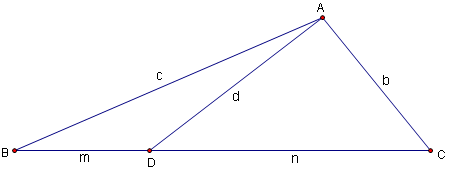
\includegraphics[width=9cm]{images/Stewarts_theorem.png}
\end{figure}

\subsection{Ceva and Menelaus}
\begin{thrm}{Ceva's Theorem}{} 
Given a triangle $\Delta ABC $ with a point $P$ inside the triangle, continue lines $AP$, $BP$, $CP$ to intersect $BC$, $CA$, $AB$ at $D$, $E$, $F$ respectively. 
\begin{equation} \frac {AF}{FB} \times \frac {BD}{DC} \times \frac {CE}{EA} = 1 \end{equation} 
\end{thrm}

\begin{figure}[H]
    \centering
    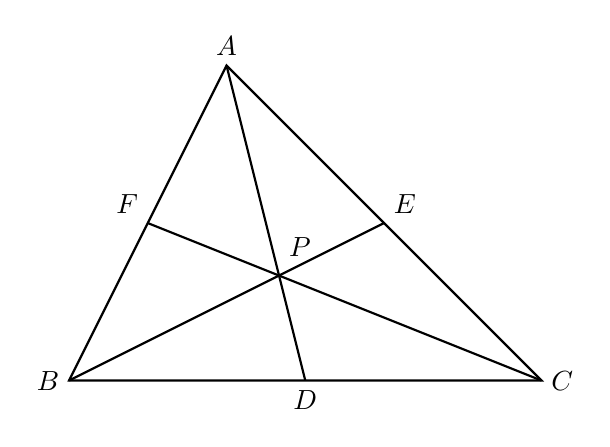
\begin{tikzpicture}
    \coordinate[label=left:$B$] (B) at (0,0) {};
    \coordinate[label=right:$C$] (C) at (6,0) {};
    \coordinate[label=above:$A$] (A) at (2,4) {};
    \draw [thick] (A) -- (B) -- (C) -- cycle;
    \coordinate[label=below:$D$] (D) at (3,0) {};
    \coordinate[label=30:$E$] (E) at (4,2) {};
    \coordinate[label=150:$F$] (F) at (1,2) {};
    \draw [thick] (A) -- (D);
    \draw [thick] (B) -- (E);
    \draw [thick] (C) -- (F);
    \node [label=80:$P$] at (2.65,1.33) {};
    \end{tikzpicture}
\end{figure}

\begin{thrm}{Menelaus' Theorem}{}
Given a triangle $\Delta ABC$, and a transversal that intersects $BC$, $AC$, $AB$ at points $D$, $E$, $F$ respectively. 
\begin{equation} \frac {AF}{FB} \times \frac {BD}{DC} \times \frac {CE}{EA} = 1 \end{equation} 
\end{thrm}

\begin{figure}[H]
    \centering
    \begin{tikzpicture}
    \coordinate[label=240:$C$] (C) at (0,0) {};
    \coordinate[label=below:$B$] (B) at (5,0) {};
    \coordinate[label=above:$A$] (A) at (2,4) {};
    \coordinate[label=-60:$D$] (D) at (9,0) {};
    \coordinate[label=135:$E$] (E) at (1,2) {};
    \draw (A) -- (B);
    \draw (C) -- (D);
    \draw (A) -- (C);
    \draw (D) -- (E);
    \node [label=80:$F$] at (4,1.33) {};
    \end{tikzpicture}
\end{figure}
\pagebreak

\section{Quadrilaterals}
\begin{thrm}{British Flag Theorem}{} 
If $ABCD$ is a rectangle and $P$ is a point inside of it, then we have 
\[ PA^2 + PC^2 = PB^2 + PD^2 \] 
\end{thrm}

\begin{figure}[H]
    \centering
    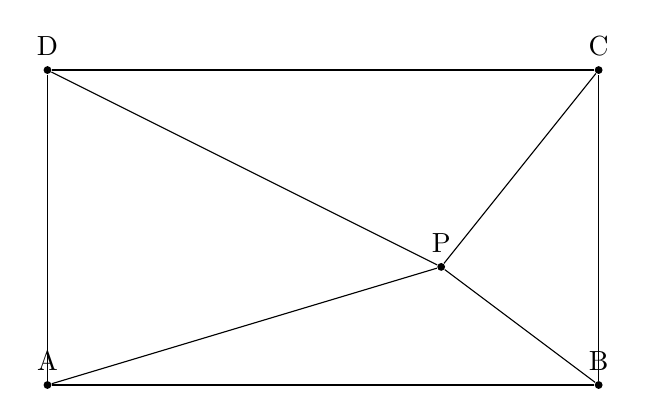
\begin{tikzpicture}[dot/.style={circle,inner sep=1pt,fill,label={#1},name=#1},
  extended line/.style={shorten >=-#1,shorten <=-#1},
  extended line/.default=1cm]
        \node [dot=A] at (0,0) {};
        \node [dot=B] at (7,0) {};
        \node [dot=C] at (7,4) {};
        \node [dot=D] at (0,4) {};
        \node [dot=P] at (5,1.5) {};
        \draw (A) -- (B) -- (C) -- (D) -- (A);
        \draw (P) -- (A);
        \draw (P) -- (B);
        \draw (P) -- (C);
        \draw (P) -- (D);
    \end{tikzpicture}
\end{figure}

\begin{proof}
This can be easily proven using Pythagoras' Theorem.
\end{proof}
\pagebreak

\section{Circle}
The reader should be familiar with basic circle terminology, such as \textbf{center}, \textbf{radius}, \textbf{chord}, \textbf{diameter}, \textbf{tangent}, \textbf{secant}, \textbf{arc}, \textbf{sector}, \textbf{segment}, and \textbf{circumference}.

\subsection{Angles}
Angle subtended at the centre of a circle by a chord is twice the angle subtended on the circumference.

All angles subtended by a fixed chord in the same segment of a circle are equal.

\subsection{Cyclic Quadrilaterals}
Angle chasing and cyclic quadrilaterals
\begin{thrm}{Ptolemy's Theorem}{}
Given a cyclic quadrilateral $ABCD$, the product of lengths of diagonals is equal to the sum of products of lengths of the pairs of the opposite sides: 
\begin{equation} AC \cdot BD = AB \cdot CD + AD \cdot BC \end{equation} 
\end{thrm}

\begin{figure}[H]
    \centering
    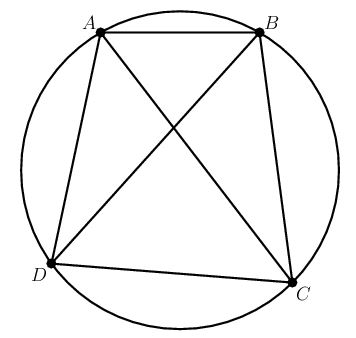
\includegraphics[width=6cm]{images/Ptolemys_theorem.jpg}
\end{figure}

\begin{thrm}{Ptolemy's Inequality}{}
For four points $A, B, C, D$ in the plane,
\begin{equation}
AB \cdot CD + BC \cdot DA \ge AC \cdot BD
\end{equation}
where equality holds if and only if $ABCD$ is a cyclic quadrilateral with diagonals $AC$ and $BD$, or if $A, B, C, D$ are collinear.
\end{thrm}

\begin{proof}
We construct a point $P$ such that the triangles $APB$ and $DCB$ are similar and have the same orientation. This means that
\begin{equation} \tag{1}
BD = \frac{BA \cdot DC}{AP}
\end{equation}

But since this is a spiral similarity, we also know that the triangles $ABD$ and $PBC$ are also similar, which implies that
\begin{equation} \tag{2}
BD = \frac{BC \cdot AD}{PC}
\end{equation}

By the triangle inequality, we have $AP + PC \ge AC$. Multiplying both sides of the inequality by $BD$ and using equations $(1)$ and $(2)$ gives us
\[ BA \cdot DC + BC \cdot AD \ge AC \cdot BD \]

which is the desired inequality. Equality holds iff $A$, $P$, $C$ are collinear. But since the triangles $BAP$ and $BDC$ are similar, this would imply that the angles $BAC$ and $BDC$ are congruent, i.e. that $ABCD$ is a cyclic quadrilateral.
\end{proof}

\begin{thrm}{Brahmagupta's Formula}{} 
Given a cyclic quadrilateral $ABCD$, \begin{equation} [ABCD] = \sqrt{(s-a)(s-b)(s-c)(s-d)} \end{equation} where $s$ denotes the semiperimeter. \end{thrm}
\pagebreak

\subsection{Power of a Point}
\textbf{Power of a point} is a frequently used tool in Olympiad geometry.

\begin{thrm}{Power of a point}{}
Let $\Gamma$ be a circle, and $P$ be a point. Let a line through $P$ meet $\Gamma$ at points $A$ and $B$, and another line through $P$ meet $\Gamma$ at points $C$ and $D$. Then 
\begin{equation}
PA \cdot PB = PC \cdot PD
\end{equation} 
\end{thrm}

\begin{figure}[H]
    \centering
    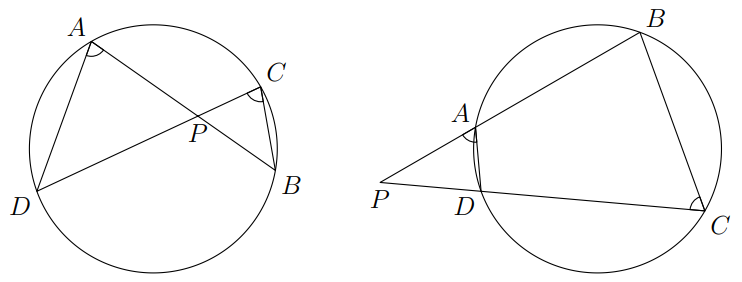
\includegraphics[width=12cm]{images/Power_of_a_point.png}
\end{figure}

\begin{proof}
There are two configurations to consider, depending on whether $P$ lies inside the circle or outside the circle.

When $P$ lies inside the circle, we have $\angle PAD = \angle PCB$ and $\angle APD = \angle CPB$, so triangles $PAD$ and $PCB$ are similar. Hence $\dfrac{PA}{PD} = \dfrac{PC}{PB}$. Rearranging, we get $PA \cdot PB = PC \cdot PD$.

When $P$ lies outside the circle, we have $\angle PAD = \angle PCB$ and $\angle APD = \angle CPB$, so again triangles $PAD$ and $PCB$ are similar. We get the same result in this case.
\end{proof}

As a special case, when $P$ lies outside the circle and $C=D$($PC$ is a tangent), we have \begin{equation} PA \cdot PB = PC^2 \end{equation}

\begin{figure}[H]
    \centering
    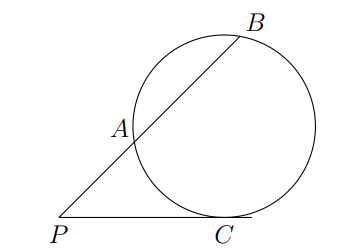
\includegraphics[width=6cm]{images/Power_of_a_point2.png}
\end{figure}
\pagebreak

\begin{thrm}{Converse to Power of a Point}{}
Let $A, B, C, D$ be four distinct points. Let lines $AB$ and $CD$ intersect at $P$. Assume that either (1) $P$ lies on both line segments $AB$ and $CD$, or (2) $P$ lies on neither line segments. Then $A, B, C, D$ are concyclic if and only if $PA \cdot PB = PC \cdot PD$.
\end{thrm}

\begin{proof}
The expression $PA \cdot PB = PC \cdot PD$ can be rearranged as $\dfrac{PA}{PD} = \dfrac{PC}{PB}$. In both configurations described in the statement of the theorem, we have $\angle APD = \angle CPB$. It follows by angles and ratios that triangles $APD$ and $CPB$ are similar.

Thus $\angle PAD = \angle PCB$. In both cases this implies that $A, B, C, D$ are concyclic.
\end{proof}

Suppose that $\Gamma$ has center $O$ and radius $r$. We say that the \textbf{power} of point $P$ with respect to $\Gamma$ is
\[ PO^2 - r^2 \]

Let line $PO$ meet $\Gamma$ at points $A$ and $B$, so that $AB$ is a diameter. We will use \emph{directed lengths}, meaning that for collinear points $P, A, B$, an expression such as $PA \cdot PB$ is assigned a positive value if $PA$ and $PB$ point in the same direction, and a negative value if they point in opposite directions. Then
\[ PA \cdot P B = (PO + OA)(PO + OB) = (PO-r)(PO+r) = PO^2 - r^2, \]
which is the power of $P$. So the power of a point theorem says that this quantity equals to $PC \cdot PD$, where $C$ and $D$ are the intersections with $\Gamma$ of any line through $P$.

By convention, the power of $P$ is negative when $P$ is inside the circle, and positive when $P$
is outside the circle. When $P$ is outside the circle, the power equals to the square of the length
of the tangent from $P$ to the circle.

\begin{figure}[H]
    \centering
    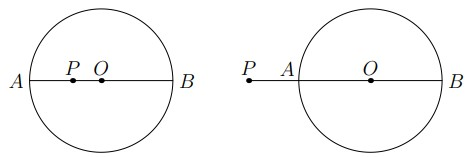
\includegraphics[width=8cm]{images/Power_of_a_point3.jpg}
\end{figure}

Let $\Gamma_1$ and $\Gamma_2$ be two circles with different centers $O_1$ and $O_2$, and radii $r_1$ and r$_2$ respectively.

The radical axis of $\Gamma_1$ and $\Gamma_2$ is the set of points with equal powers with respect to both circles.
\[ {PO_1}^2 - {r_1}^2 = {PO_2}^2 - {r_2}^2 \]
which can be represented as 
\[ pow(P, \Gamma_1) = pow(P, \Gamma_2). \]

The radical axis is a line perpendicular to the line connecting the circles' centers (line $\ell$).
\begin{proof}
\begin{lemma}
Let $P$ be a point in the plane, and let $P'$ be the foot of the perpendicular from $P$ to $O_1O_2$. Then \[ pow(P, \Gamma_1) - pow(P, \Gamma_2) = pow(P', \Gamma_1) - pow(P', \Gamma_2). \]
\end{lemma}
The proof of the lemma is an easy application of the Pythagorean Theorem.

\begin{lemma}
There is a unique point $P$ on line $O_1O_2$ such that $pow(P, O_1) = pow(P, O_2)$.
\end{lemma}

Proof: First show that $P$ lies between $O_1$ and $O_2$ via proof by contradiction, by using a bit of inequality theory and the fact that $O_1O_2 > r_1 + r_2$. Then, use the fact that $O_1P + PO_2 = O_1O_2$ (a constant) to prove the lemma.

The first lemma shows that every point on the plane can be equivalently mapped to a line on $O_1O_2$. The second lemma shows that only one point in this mapping satisfies the given condition. Combining these two lemmas shows that the radical axis is a line perpendicular to $\ell$, hence proved.
\end{proof}

When $\Gamma_1$ and $\Gamma_2$ intersect, the intersection points $A$ and $B$ both have a power of $0$ with respect to either circle, so $A$ and $B$ must lie on the radical axis. This shows that the radical axis \emph{coincides with the common chord} when the circles intersect.

To show that some point lies on the radical axis or the common chord, we can show that the point has \emph{equal powers with respect to the two circles}.

\begin{figure}[H]
    \centering
    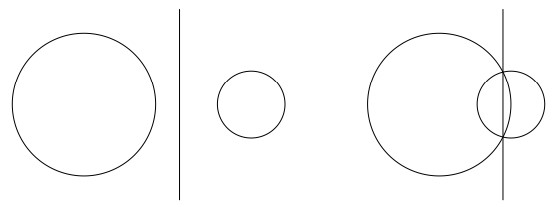
\includegraphics[width=10cm]{images/Radical_axis.jpg}
    \caption{Radical axis}
\end{figure}

\begin{figure}[H]
    \centering
    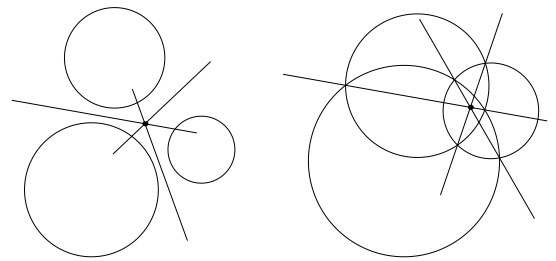
\includegraphics[width=10cm]{images/Radical_center.jpg}
    \caption{Radical center}
\end{figure}

\begin{thrm}{Radical Axis Theorem}{}
Given three circles, no two concentric, the three pairwise radical axes (which are non-parallel) are concurrent, at a point known as the radical center.
\end{thrm}

\begin{proof}
Denote the three circles by $\Gamma_1, \Gamma_2, \Gamma_3$, and denote the radical axes of $\Gamma_i$ and $\Gamma_j$ by $\ell_{ij}$.

Suppose that the radical axes are not all parallel. Let $\ell_{12}$ and $\ell_{13}$ meet at $X$. Since $X$ lies on $\ell_{12}$, it has equal powers with respect to $\Gamma_1$ and $\Gamma_2$. Since X lies on $\ell_{13}$, it has equal powers with respect to $\Gamma_1$ and $\Gamma_3$. Therefore, $X$ has equal powers with respect to all three circles, and hence it must lie on $\ell_{23}$ as well.
\end{proof}

\subsection{Euler's Line and Nine-point Circle}
\begin{thrm}{Hamilton's theorem}{}
For $\triangle ABC$ with circumcenter $O$ and orthocenter $H$,
\[ \overrightarrow{OH} = \overrightarrow{OA} + \overrightarrow{OB} + \overrightarrow{OC} \]
\end{thrm}

\begin{thrm}{Euler line}{}
The circumcenter $O$, the centroid $G$ and the orthocenter $H$ are collinear.

In fact, we have 
\[ GH=2 OG \]
and
\[ OI^2 = R^2-2Rr \]
\end{thrm}

\begin{thrm}{Nine-point circle}{}
The midpoints of each side of the triangle, the feet of each altitude, and the midpoints of the line segments from each vertex to the orthocenter, all lie on a single circle.
\end{thrm}

The center of this circle lies on the Euler line, at the midpoint between the orthocenter and circumcenter.

The radius of this circle is half the circumradius of the triangle.

\subsection{Simson line}
\subsection{Miquel's theorem}
\begin{thrm}{Miquel's theorem}{}
Let $ABC$ be a triangle, and let $X, Y, Z$ be points on lines $BC, CA, AB$ respectively. Assume that the six points $A, B, C, X, Y, Z$ are all distinct. Then the circumcircles of triangles $AYZ, BZX, CXY$ pass through a common point.
\end{thrm}

\begin{proof}
The proof involves angle chasing.
\end{proof}

\pagebreak


\section*{Problems}
\begin{prbm}[Oxford MAT 2022]
100 circles all share the same centre, the $n$-th circle named as $C_n$. For each whole number $n$ between 1 and 99 inclusive, a tangent to circle $C_n$ intersects circle $C_{n+1}$ at two points, separated by a distance of 2.

Given that $C_1$ has radius 1, what is the radius of $C_{100}$?
\end{prbm}

\begin{proof}[Solution]
The relationship between circle $C_n$ of radius $r_n$ and circle $C_{n+1}$ of radius $r_{n+1}$ is shown below.
\begin{figure}[H]
    \centering
    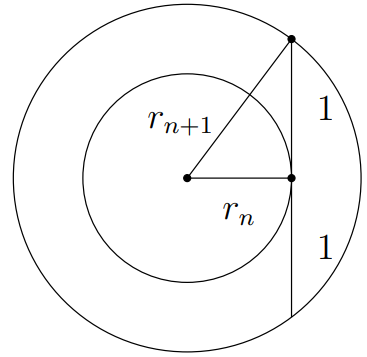
\includegraphics[width=6cm]{images/c_n_circles.png}
\end{figure}

The tangent is at right angles to the radius, so there is a right-angled triangle with hypotenuse $r_n+1$ and other sides $r_n$ and $1$. Pythagoras gives ${r_{n+1}}^2 = {r_n}^2 + 1$. Since ${r_1}^2 = 1$, we have ${r_2}^2 = 2$ and ${r_3}^2 = 3$ and so on, up to ${r_{100}}^2 = 100$, so the radius of $C_100$ is 10.
\end{proof}
\pagebreak

\begin{prbm}
Prove that for angles $\alpha_1, \alpha_2, \dots, \alpha_n$ which satisfy the condition $0\degree \le a_i \le 180\degree$ for $i=1,2,\dots,n$ then
\[ \sin\alpha_1 + \sin\alpha_2 + \cdots + \sin\alpha_n \le n \sin\frac{\alpha_1+\cdots+\alpha_n}{n} \]
with equality iff $\alpha_1 = \cdots = \alpha_n$.
\end{prbm}

\begin{proof}
For 2 angles, 

\end{proof}

\chapter{Trigonometry}
\textbf{Readings:}
\begin{itemize}
\item \href{https://www.ams.org/books/prb/025/prb025-endmatter.pdf}{AMS}
\item \href{https://mathematicalolympiads.files.wordpress.com/2012/08/103-trigonometry-problems-titu-andreescu-zuming-feng.pdf}{Problems}
\end{itemize}

\section{Basic Definitions}
\textbf{Trigonometric functions} describe how the ratio of lengths vary according to the angle between the lengths.

For a triangle $\triangle ABC$ with $\angle C=90\degree$, we define \textbf{sine} as
\begin{equation}
\sin A=\frac{a}{c}
\end{equation}
and \textbf{cosine} as
\begin{equation}
\cos A=\frac{b}{c}.
\end{equation}
We define \textbf{tangent} as the ratio of sine and cosine; that is,
\begin{equation}
\tan A=\frac{\sin A}{\cos A}=\frac{a}{b}.
\end{equation}
We also define the reciprocals of the above trigonometric functions: \textbf{cosecant}, \textbf{secant} and \textbf{cotangent} are the reciprocals of sine, cosine and tangent respectively.
\begin{equation}
\cosec A=\frac{1}{\sin A}
\end{equation}
\begin{equation}
\sec A=\frac{1}{\cos A}
\end{equation}
\begin{equation}
\cot A=\frac{1}{\tan A}
\end{equation}

\section{Formulae}
\subsection{Pythagorean identities}
The following equation is known as the \textbf{Pythagorean identity}.
\begin{equation}\label{pythagorean_identity}
\sin^2 A + \cos^2 A = 1
\end{equation}
\begin{proof}
\[ \sin^2A+\cos^2A=\brac{\frac{a}{c}}^2+\brac{\frac{b}{c}}^2=\frac{a^2+b^2}{c^2} \]
By Pythagoras' Theorem, for a right-angled triangle, $a^2+b^2=c^2$. Hence we have our desired result.
\end{proof}
The following two equations are corollaries of \cref{pythagorean_identity}; they can be easily derived and shall be left as an exercise for the reader.
\[ \tan^2 A + 1 = \sec^2 A \]
\[ 1 + \cot^2 A = \cosec^2 A \]

\begin{exmp}{}{}
Compute $\sin^25\degree+\sin^210\degree+\cdots+\sin^290\degree$.
\end{exmp}
\begin{solution}
\begin{align*}
&\sin^25\degree+\sin^210\degree+\cdots+\sin^290\degree \\
&= (\sin^25\degree+\sin^285\degree) + \cdots + (\sin^240\degree+\sin^250\degree)+\sin^245\degree+\sin^290\degree \\
&= (\sin^25\degree+\cos^25\degree) + \cdots + (\sin^240\degree+\cos^240\degree)+\frac{1}{2}+1 \\
&= 8(1)+\frac{1}{2}+1 \\
&= \boxed{9\frac{1}{2}}
\end{align*}
\end{solution}

\subsection{Addition formulae}
\[ \sin (A \pm B) = \sin A \cos B \pm \cos A \sin B \]
\[ \cos (A \pm B) = \cos A \cos B \mp \sin A \sin B \]
\[ \tan (A \pm B) = \frac{\tan A \pm \tan B}{1 \mp \tan A \tan B} \]

\subsubsection{Double-angle formulae}
\[ \sin 2A = 2 \sin A \cos A \]
\[ \begin{split}
\cos 2A &= \cos^2 A - \sin^2 A \\
&= 2 \cos^2 A - 2 \\
&= 2 - 2 \sin^2 A
\end{split} \]
\[ \tan 2A = \frac{2 \tan A}{1 - \tan^2 A} \]

\subsubsection{Triple-angle formulae}
\[ \sin 3A = 3 \sin A - 4 \sin^3 A \]
\[ \cos 3A = 4 \cos^3 A- 3 \cos A \]
\[ \tan 3A = \frac{3\tan A-\tan^3A}{1-3\tan^2A} \]

\subsubsection{Half-angle formulae}
The following formulae are corollaries of \cref{pythagorean_identity}.
\[ \sin \frac{A}{2} = \pm \sqrt{\frac{1-\cos A}{2}} \]
\[ \cos \frac{A}{2} = \pm \sqrt{\frac{1+\cos A}{2}} \]

\subsubsection{Multiple-angle formulae}
Multiple-angle formulas are given by
\[ \sin nA = \sum_{k=0}^n \binom{n}{k} \cos^kA \sin^{n-k}A \sin\frac{n-k}{2}\pi \]
\[ \cos nA = \sum_{k=0}^n \binom{n}{k} \cos^kA \sin^{n-k}A \cos\frac{n-k}{2}\pi \]

\subsubsection{Sum to product}
\[ \sin A + \sin B = 2 \sin \frac{A+B}{2} \cos \frac{A-B}{2} \]
\[ \sin A - \sin B = 2 \cos \frac{A+B}{2} \sin \frac{A-B}{2} \]
\[ \cos A + \cos B = 2 \cos \frac{A+B}{2} \cos \frac{A-B}{2} \]
\[ \cos A - \cos B = -2 \sin \frac{A+B}{2} \sin \frac{A-B}{2} \]

\subsubsection{Product to sum}
\[ \sin A \cos B = \frac{1}{2}\sqbrac{\sin(A+B)+\sin(A-B)} \]
\[ \cos A \cos B = \frac{1}{2}\sqbrac{\cos(A+B)+\cos(A-B)} \]
\[ \sin A \sin B = -\frac{1}{2}\sqbrac{\cos(A+B)-\cos(A-B)} \]

\subsection{R-formula}
\[ a \sin \theta \pm b \cos \theta = \sin (\theta \pm \alpha) \]
\[ a \cos \theta \mp b \cos \theta = \cos (\theta \pm \alpha) \]
where $R = \sqrt{a^2 + b^2}$,
$\alpha = \tan^{-1} \dfrac{b}{a}$ where $0 < \alpha < \frac{\pi}{4}$.

\section{Theorems}
\begin{thrm}{Sine rule}{} 
\begin{equation}
\frac{a}{\sin A} = \frac{b}{\sin B} = \frac{c}{\sin C} = 2R
\end{equation} 
where $R$ denotes radius of circumcircle of triangle $ABC$. 
\end{thrm}

\begin{thrm}{Cosine rule}{} 
\begin{equation}
a^2 = b^2 + c^2 - 2bc \cos A
\end{equation} 
\end{thrm}

\begin{thrm}{Tangent law}{}
\begin{equation}
\frac{a-b}{a+b}=\frac{\tan\frac{A-B}{2}}{\tan\frac{A+B}{2}}
\end{equation}
\end{thrm}

\begin{thrm}{Cotangent law}{}
\begin{equation}
\cot A=\frac{b^2+c^2-a^2}{4S}
\end{equation}
\end{thrm}
\pagebreak

\section{Hyperbolic Functions}
\subsection{Basics}
The three main hyperbolic functions are:
\begin{equation}
\sinh x = \frac{e^x-e^{-x}}{2}
\end{equation}
\begin{equation}
\cosh x = \frac{e^x+e^{-x}}{2}
\end{equation}
\begin{equation}
\tanh x = \frac{e^x-e^{-x}}{e^x+e^{-x}} = \frac{e^{2x}-1}{e^{2x}+1}
\end{equation}

It is easy to see that
\[ \sinh x + \cosh x = e^x \]

\subsection{Reciprocals and Inverses}
Again these functions all have their inverse functions:
\begin{equation}
\sinh^{-1} x = \arsinh x = \ln(x+\sqrt{x^2+1})
\end{equation}
$\arsinh x$ has domain $x \ge 1$.

\begin{equation}
\cosh^{-1} x = \arcosh x = \ln(x+\sqrt{x^2-1})
\end{equation}
$\arcosh x$ has domain $x \ge 1$.

\begin{equation}
\tanh^{-1} x = \artanh x = \frac{1}{2}\ln(1+x)-\frac{1}{2}\ln(1-x)
\end{equation}
$\artanh x$ has domain $-1<x<1$.

As well as their reciprocal functions:
\begin{equation}
\cosech x = \frac{1}{\sinh x}
\end{equation}
\begin{equation}
\sech x = \frac{1}{\cosh x}
\end{equation}
\begin{equation}
\coth x = \frac{1}{\tanh x}
\end{equation}

\subsection{Identities}
Hyperbolic function identities have very similar forms to the trigonometric identities. 

However there is one key difference outlined in \textbf{Osborn's rule}: all the identities for the hyperbolic functions are exactly the same as the trigonometric identities, except whenever a product of two $\sinh$ functions is present we put a minus sign in front. For example if a trigonometric formula involved a $\sin^2x$, then the corresponding hyperbolic formula would contain a $-\sinh^2x$ instead.

\begin{table}[H]
\centering
\begin{tabular}{c|c}
\hline\hline
Trigonometric & Hyperbolic \\
\hline
$\cos^2\theta + \sin^2\theta = 1$ & $\cosh^2x - \sinh^2x = 1$ \\
$\sin(A \pm B) = \sin A \cos B \pm \cos A \sin B$ & $\sinh(A \pm B) = \sinh A \cosh B \pm \cosh A \sinh B$ \\
$\cos(A \pm B) = \cos A \cos B \mp \sin A \sin B$ & $\cosh(A \pm B) = \cosh A \cosh B \mp \sinh A \sinh B$ \\
$\cos 2\theta = \cos^2\theta - \sin^2\theta$ & $\cosh 2\theta = \cosh^2\theta + \sinh^2\theta$ \\
$\sin 2\theta = 2 \sin\theta \cos\theta$ & $\sinh 2\theta = 2 \sinh\theta \cosh\theta$ \\
$1 + \tan^2\theta = \sec^2\theta$ & $1 - \tanh^2\theta = \sech^2\theta$ \\
$1 + \cot^2\theta = \cosec^2\theta$ & $1 - \coth^2\theta = - \cosech^2\theta$ \\
\hline\hline
\end{tabular}
\end{table}
\pagebreak

\section*{Problems}
\begin{prbm}
Angles of $\triangle ABC$ satisfies
\[ \frac{\sin A+\sin B+\sin C}{\cos A+\cos B+\cos C}=\frac{12}{7} \]
and
\[ \sin A\sin B\sin C=\frac{12}{15}. \]
Given that $\sin C$ takes on three possible values $s_1,s_2,s_3$, find the value of $s_1s_2s_3$.
\end{prbm}
\begin{solution} \
\begin{align*}
\sin A+\sin B+\sin C
&= 2\sin\frac{A+B}{2}\cos\frac{A-B}{2}+\sin C \\
&= 2\sin\brac{90\degree-\frac{C}{2}}\cos\frac{A-B}{2}+2\sin\frac{C}{2}\cos\frac{C}{2} \\
&= 2\cos\frac{C}{2}\cos\frac{A-B}{2}+2\sin\frac{C}{2}\cos\frac{C}{2} \\
&= 2\cos\frac{C}{2}\brac{\cos\frac{A-B}{2}+\cos\frac{A+B}{2}} \\
&= 2\cos\frac{C}{2}\brac{2\cos\frac{A}{2}\cos\frac{B}{2}} 
= 4\cos\frac{A}{2}\cos\frac{B}{2}\cos\frac{C}{2}
\end{align*}
and
\begin{align*}
\cos A+\cos B+\cos C
&= 2\cos\frac{A+B}{2}\cos\frac{A-B}{2}+\cos C \\
&= 2\cos\brac{90\degree-\frac{C}{2}}\cos\frac{A-B}{2}+\cos2\brac{\frac{C}{2}} \\
&= 2\sin\frac{C}{2}\cos\frac{A-B}{2}+\brac{1-2\sin^2\frac{C}{2}} \\
&= 1+2\sin\frac{C}{2}\brac{\cos\frac{A-B}{2}-\sin\frac{C}{2}} \\
&= 1+2\sin\frac{C}{2}\brac{\cos\frac{A-B}{2}-\sin\brac{90\degree-\frac{A+B}{2}}} \\
&= 1+2\sin\frac{C}{2}\brac{\cos\frac{A-B}{2}-\cos\frac{A+B}{2}} \\
&= 1+2\sin\frac{C}{2}\brac{2\sin\frac{A}{2}\sin\frac{B}{2}} 
= 1+4\sin\frac{A}{2}\sin\frac{B}{2}\sin\frac{C}{2}
\end{align*}

This gives us the following simultaneous equations.
\[ \begin{cases}
\dfrac{\sin A+\sin B+\sin C}{\cos A+\cos B+\cos C} = \dfrac{4\cos\frac{A}{2}\cos\frac{B}{2}\cos\frac{C}{2}}{1+4\sin\frac{A}{2}\sin\frac{B}{2}\sin\frac{C}{2}} = \dfrac{12}{7} \\
\sin A\sin B\sin C = 8\brac{\sin\dfrac{A}{2}\sin\dfrac{B}{2}\sin\dfrac{C}{2}}\brac{\cos\dfrac{A}{2}\cos\dfrac{B}{2}\cos\dfrac{C}{2}} = \dfrac{12}{15}
\end{cases} \]

Solving, we get
\[ \begin{cases}
\sin\dfrac{A}{2}\sin\dfrac{B}{2}\sin\dfrac{C}{2}=\dfrac{1}{10} \\
\cos\dfrac{A}{2}\cos\dfrac{B}{2}\cos\dfrac{C}{2}=\dfrac{3}{5}
\end{cases} \]

We see that
\begin{align*}
\sin\frac{C}{2} &= \cos\frac{A+B}{2} = \cos\frac{A}{2}\cos\frac{B}{2} - \sin\frac{A}{2}\sin\frac{B}{2} \\
\sin^2\frac{C}{2}\cos\frac{C}{2} &= \frac{3}{5}\sin\frac{C}{2} - \frac{1}{10}\cos\frac{C}{2}
\end{align*}

Let $t=\cos\dfrac{C}{2}$. Then we get a quadratic equation. Solving it gives us 
\[ t=\sqrt{\frac{1}{2}}, \quad t=\sqrt{\frac{4}{5}}, \quad t=\sqrt{\frac{3}{10}}. \]

Hence $\boxed{s_1=1, s_2=\dfrac{4}{5}, s_3=\dfrac{3}{5}}$.
\end{solution}
\pagebreak

\begin{prbm}
Let 
\[ A = \cos^2 10\degree+\cos^2 50\degree - \sin40\degree\sin80\degree. \]
Determine the value of $A$.
\end{prbm}
\begin{solution}
Let $B=\sin^210\degree+\sin^250\degree-\cos40\degree\cos80\degree$.

Then
\begin{align*}
A+B &= 2-\cos40\degree \\
A-B &= (\cos^210\degree-\sin10\degree) + (\cos^250\degree-\sin^250\degree) + (\cos40\degree\cos80\degree-\sin40\degree\sin80\degree) \\
&= \cos20\degree + \cos100\degree + \cos(40\degree+80\degree) \\
&= \cos20\degree + \cos100\degree + \cos120\degree \\
&= 2\cos60\degree\cos40\degree - \cos60\degree \\
&= \cos40\degree - \frac{1}{2}
\end{align*}
Adding up the two equations gives us $2A=\dfrac{3}{2}$. Hence $\boxed{A=\dfrac{3}{4}}$.
\end{solution}
\pagebreak

\begin{prbm}[SMO Open]
Find the value of
\[ \frac{\tan40\degree\tan60\degree\tan80\degree}{\tan40\degree+\tan60\degree+\tan80\degree}. \]
\end{prbm}
\begin{solution}
We can show, more generally, that an acute $\triangle ABC$,
\[ \frac{\tan A\tan B\tan C}{\tan A+\tan B+\tan C}=1. \]
We see that
\begin{align*}
\tan A+\tan B+\tan 
&= \tan A+\tan B+\tan[180\degree-(A+B)] \\
&= \tan A+\tan B-\tan(A+B) \\
&= \tan A+\tan B-\frac{\tan A+\tan B}{1-\tan A\tan B} \\
&= (\tan A+\tan B)\brac{1-\frac{1}{1-\tan A\tan B}} \\
&= (\tan A+\tan B)\brac{-\frac{\tan A\tan B}{1-\tan A\tan B}} \\
&= \tan A\tan B\brac{-\frac{\tan A+\tan B}{1-\tan A\tan B}} \\
&= \tan A\tan B[-\tan(A+B)] \\
&= \tan A\tan B\tan[180\degree-(A+B)] \\
&= \tan A\tan B\tan C
\end{align*}
Hence proven.
\end{solution}
\pagebreak

\begin{prbm}[Oxford MAT]
Evaluate 
\[ \sin^2 1\degree + \sin^2 2\degree + \dots + \sin^2 89\degree + \sin^2 90\degree. \]
\end{prbm}

\begin{proof}[Solution]
Recall the Pythagorean Identity $\sin^2 x + \cos^2 x = 1$.

Rewriting and pairing up terms gives us 
\begin{align*}
&\sin^2 1\degree + \sin^2 2\degree + \dots + \cos^2 2\degree + \cos^2 1\degree + 1 \\
&= (\sin^2 1\degree + \cos^2 1\degree) + \dots + (\sin^2 44\degree + \cos^2 44\degree) + \sin^2 45\degree + 1 \\
&= 44(1) + \frac{1}{2} + 1 = \boxed{45\frac{1}{2}}
\end{align*}
\end{proof}

\chapter{Coordinate Systems}
\section{Cartesian Coordinates}
\subsection{Basics}
The coordinate plane is determined by two \textbf{axes} -- a horizontal $x$-axis and a vertical $y$-axis; both axes intersect at a point called the \textbf{origin}. Each point in the coordinate plane can be specified by an ordered pair of numbers $(x,y)$.

The \textbf{gradient} of a line with points $(x_1, y_1)$ and $(x_2, y_2)$ is given by
\begin{equation}
m = \frac{y_2-y_1}{x_2-x_1}
\end{equation}

Given gradient $m$ and $y$-intercept $c$, a line can be represented in the point-slope form:
\begin{equation}
y=mx+c
\end{equation}

Given gradient $m$ and a point on the line $(x_1,y_1)$, a line can be represented as
\begin{equation}
y-y_1=m(x-x_1)
\end{equation}

For two \textbf{parallel} lines, they have the same gradients.

For two \textbf{perpendicular} lines, the product of the gradients is $-1$.

The distance from a point $(m, n)$ to the line $Ax + By + C = 0$ is given by
\[ d = \frac{Am+Bn+C}{\sqrt{A^2+B^2}} \]

The distance between two lines is given by


The area of polygon is given by


reflection of point, line about line

\subsection{Conic Sections}
Definitions and basic properties of conic sections - refer to F maths
\subsubsection{Standard Equations of Conics}
Conic sections are the family of curves obtained by intersecting a cone with a plane. This intersection can take different forms according to the angle the intersecting plane makes with the side of the cone. The standard conic sections are the circle, the parabola, the ellipse and the hyperbola. There are also special cases, such as a point or a line, however these are trivial (sometimes called degenerate) so we shall not cover them.

\begin{table}[H]
\centering
\renewcommand{\arraystretch}{1.8}
\begin{tabular}{c|c|c}
\hline\hline
Conic & Cartesian equation & Parametric equation \\
\hline
Circle & $x^2+y^2=a^2$ & $x=\cos t, y=\sin t$ \\
Parabola & $x=4ay^2$ & $x=4at^2, y=t$ \\
Ellipse & $\frac{x^2}{a^2}+\frac{y^2}{b^2}=1$ & $x=a\cos t, y=b\sin t$ \\
Hyperbola & $\frac{x^2}{a^2}-\frac{y^2}{b^2}=1$ & $x=b\tan t, y=a\sec t$ \\
\hline\hline
\end{tabular}
\end{table}

\begin{remark}
The circle is a special case of the ellipse, where $a=b$.
\end{remark}

\subsubsection{Recognising Conics}
The general equation of any conic is $Ax^2 + Bxy + Cy^2 + Dx + Ey + F = 0$. When we see an equation like this we know that it describes a conic, but to find out which conic it describes one has to manipulate the equation into one of the equations given above.

One method is to sketch a phase plot which is a graph drawn up from the given equation to allow us to try understand what the equation describes in a physical system. In many cases we can manipulate the given equation to take the form of a conic.
\pagebreak

\section{Polar Coordinates}
You will already be familiar with coordinates in the form $(x, y)$ meaning that we move $x$ units in the $x$-direction (along the $x$-axis) and $y$ in the $y$-direction (along the $y$-axis). These are Cartesian coordinates on the $xy$-plane. Although Cartesian coordinates are very useful, there are sometimes situations where it is much easier to use another coordinate system called \textbf{polar coordinates}. These are coordinates in the form $(r,\theta)$ where $r$ is the distance to the point from the origin and $\theta$ is the angle in radians between the positive $x$-axis and the line formed by $r$.

From trigonometry and Pythagoras' theorem there are the following relationships:
\[ x = r\cos\theta \quad y = r\sin\theta \quad r = \sqrt{x^2+y^2} \]
We can use the formulae above to allow us to convert between Polar and Cartesian coordinates.

\section{Barycentric Coordinates}
\subsection{Basics}
\subsubsection{The Coordinates}
\begin{defn}{}{}
Each point in the plane is assigned an ordered triple of real numbers $P = (x, y, z)$ such that
\[ \vec{P} = x\vec{A} + y\vec{B} + z\vec{C} \quad \text{and} \quad x + y + z = 1 \]
\end{defn}
% https://web.evanchen.cc/handouts/bary/bary-full.pdf

\subsubsection{Lines}
\pagebreak

\section{Complex Numbers}

\chapter{Advanced Techniques}
\section{Inversion in the plane}
Definition and first properties
Generalised lines and circles
Inversion distance formula
O Inversive geometry

\section{Projective geometry}
Cross ratios
Projective transformations
O Projective geometry, e.g. cross ratios, harmonic bundles, poles and polars,
Pascal's theorem, and so on

\subsection{Homothety}

\section{Complete quadrilaterals}
Spiral similarity
Miquel point of a cyclic quadrilateral

